 \documentclass[a4paper,11pt]{article}

\usepackage{amsmath}
\usepackage{amssymb}
\usepackage{amsthm}
\usepackage{graphicx}
\usepackage{caption}
\usepackage{subcaption}

\newtheorem{thm}{Theorem}
\newtheorem{lem}{Lemma}

\newcommand{\beq}{\begin{equation}}
\newcommand{\eeq}{\end{equation}}

\newcommand{\ba}{\begin{array}}
\newcommand{\ea}{\end{array}}

\newcommand{\bea}{\begin{eqnarray}}
\newcommand{\eea}{\end{eqnarray}}

\newcommand{\bc}{\begin{center}}
\newcommand{\ec}{\end{center}}

\newcommand{\ds}{\displaystyle}

\newcommand{\bt}{\begin{tabular}}
\newcommand{\et}{\end{tabular}}

\newcommand{\bi}{\begin{itemize}}
\newcommand{\ei}{\end{itemize}}

\newcommand{\bd}{\begin{description}}
\newcommand{\ed}{\end{description}}

\newcommand{\bp}{\begin{pmatrix}}
\newcommand{\ep}{\end{pmatrix}}

\newcommand{\p}{\partial}
\newcommand{\sech}{\mbox{sech}}

\newcommand{\cf}{{\it cf.}~}

\newcommand{\ltwo}{L_{2}(\mathbb{R}^{2})}
\newcommand{\smooth}{C^{\infty}_{0}(\mathbb{R}^{2})}

\newcommand{\br}{{\bf r}}
\newcommand{\bk}{{\bf k}}
\newcommand{\bv}{{\bf v}}

\setlength{\textheight}{212mm}
\setlength{\textwidth}{165mm}
\topmargin -6mm
\oddsidemargin -6mm


\newcommand{\gnorm}[1]{\left|\left| #1\right|\right|}
\newcommand{\ipro}[2]{\left<#1,#2 \right>}
\title{Vortex Patches under Cnoidal Waves}
\author{Christopher W. Curtis\\
Henrik Kalisch}
\date{}
\begin{document}
\maketitle
\section*{Introduction}
\section*{Model}
Throughout, we are attempting to describe the simultaneous evolution of a free surface $y = \eta(x,t) + H$, and a compactly supported patch of vorticity $\omega(x,y,t)$ underneath the free surface.  We suppose along the curve $z=0$ that we have a solid boundary so that the normal velocity is identically zero.  In an inviscid, incompressible fluid, we can represent the fluid velocity ${\bf u}(x,y,t)$ generated by a vortex patch characterized by vorticity profile $\omega({\bf x},t)$ over the compact domain $\Omega(t)$ via the integral equation
\[
{\bf u}({\bf x},t) = \int_{\Omega(t)} {\bf K}({\bf x}-\tilde{{\bf x}})\omega(\tilde{{\bf x}},t)d\tilde{{\bf x}} + \nabla \tilde{\phi}, ~ \Delta \tilde{\phi} = 0.
\]
where $\omega$ is the vorticity, and ${\bf K}$ is the standard Biot-Savart law kernel.  The harmonic function $\tilde{\phi}$ is used to address boundary conditions as explained in \cite{saffman}.  An attractive means for discretizing this equation as summarized in \cite{cottet} is to approximate the vorticity $\omega$ by a collection of $N$ point-vortices at positions ${\bf x}_{l}(t)$ via the expansion
\begin{equation}
\omega(\tilde{{\bf x}},t) = \sum_{j=1}^{N} \frac{\Gamma_{j}}{\delta^{2}}\chi\left(\frac{\tilde{{\bf x}}-{\bf x}_{j}(t)}{\delta}\right), ~ {\bf x}_{j}(t) = \left(x_{j}(t),y_{j}(t) \right),
\label{discvort} 
\end{equation}
where $\chi$ is some appropriately chosen mollifier, see \cite{beale}, and $\Gamma_{j}$ is the circulation associated with the point vortex at ${\bf x}_{l}(t)$.  Thus, we can reduce the problem of tracking the evolution of the vortex patch to describing the motion of the point vortices via the system of ODE's
\[
\frac{d{\bf x}_{j}}{dt}  =  \sum_{l\neq j}^{N} \Gamma_{l} {\bf K}_{\delta}\left({\bf x}_{j}-{\bf x}_{l}\right) + \nabla \tilde{\phi}\left({\bf x}_{j},t\right), ~ {\bf K}_{\delta}({\bf x}) = \frac{1}{\delta^{2}}\int_{\mathbb{R}^{2}}{\bf K}({\bf x} - \tilde{\bf x})\chi \left(\frac{\tilde{{\bf x}}}{\delta} \right) d \tilde{{\bf x}}.
\]
Choosing, as in \cite{beale}, the mollifier $\chi$ to be the fourth-order kernel 
\[
\chi(r) = 2e^{-r^{2}} - \frac{1}{2}e^{-r^2/2}, 
\]
introducing periodic boundary conditions in the lateral direction and a solid boundary along the curve $z=0$ then modifies the above dynamical system to be 
\[
i\frac{d z^{\ast}_{j}}{dt}  = \frac{1}{2\pi}\left(\sum_{l\neq j}^{N} \Gamma_{l} \sum_{m=-\infty}^{\infty} \frac{\tilde{\chi}(z_{j}-z_{l}-2Lm;\delta)}{z_{j}-z_{l}-2Lm} -   \sum_{l=1}^{N} \Gamma_{l} \sum_{m=-\infty}^{\infty} \frac{\tilde{\chi}(z_{j}-z^{\ast}_{l}-2Lm;\delta)}{z_{j}-z^{\ast}_{l}-2Lm}\right)  + \p_{y}\tilde{\phi} + i\p_{x}\tilde{\phi}, 
\]
where $z_{j}=x_{j} + iy_{j}$, the period in $x$ is given by $2L$, and
\[
\tilde{\chi}(r;\delta) = \left(1-e^{-r^{2}/2\delta^{2}} \right)\left(1+2e^{-r^{2}/2\delta^{2}} \right).
\]

As can be seen, the presence of the mollifier prevents from the closed form evaluation of the sums in $m$, thereby potentially adding significant overhead in numerical computations, even if fast Fourier transforms are used to evaluate the sums.  We note however that 
\[
\tilde{\chi}(r;\delta) = 1 + \bar{\chi}(r), ~ \bar{\chi}(r) = \left(1-2e^{-r^2/2\delta^{2}} \right)e^{-r^2/2\delta^{2}}
\]
which tacitly explains the role of mollifcation, which is to remove singularities in the determination of particular velocities when $\left|z_{j}-z_{l} \right|\lesssim \delta$.  Thus, when we know that $\left|z_{j}-z_{l} \right| > \delta$, we take $\tilde{\chi}(r;\delta) \sim 1$ so that 
\[
\frac{1}{2\pi}\sum_{m=-\infty}^{\infty} \frac{\tilde{\chi}(z_{j}-z_{l}-2Lm;\delta)}{z_{j}-z_{l}-2Lm} \approx \frac{1}{4L}\cot\left(\frac{\pi}{2L}\left(z_{j}-z_{l}\right) \right),
\]
where the sum is taken in the principal value sense.  In the case that $\left|z_{j}-z_{l} \right|\lesssim \delta$, we use instead 
\[
\frac{1}{2\pi}\sum_{m=-\infty}^{\infty} \frac{\tilde{\chi}(z_{j}-z_{l}-2Lm;\delta)}{z_{j}-z_{l}-2Lm} \approx \frac{1}{4L}\cot\left(\frac{\pi}{2L}\left(z_{j}-z_{l}\right) \right) + \frac{1}{2\pi}\frac{\bar{\chi}(z_{j}-z_{l};\delta)}{z_{j}-z_{l}}.
\]
The error incurred in these approximations is only exponentially small.  We evalute the corresponding sums over the image points $z_{j}-z_{l}^{\ast}$ so as to keep the zero flow through $z=0$ condition strictly enforced.  Our use of a Fast-Multipole Method for the evaluation of the velocities $\dot{z}_{j}$ in effect determines all points either far or close to $z_{j}$, and thus the approximation above is a very natural and easy one to use in our numerical scheme.  

Following the arguments in \cite{curtis}, and again emphasizing the compact support of the vorticity $\omega(x,y,t)$, we then have at the free surface the coupled nonlinear system
\[
\eta_{t} = -\p_{x}\eta\p_{x}\tilde{\phi} + \p_{z}\tilde{\phi} + P_{v},
\]
and
\begin{multline*}
\tilde{\phi}_{t} + \frac{1}{2}\left|\nabla \tilde{\phi}\right|^{2} +\mbox{Im}\left\{Q_{v}\right\}\p_{x}\tilde{\phi} + \mbox{Re}\left\{Q_{v}\right\}\p_{z}\tilde{\phi} + g\eta = E_{v} - \frac{1}{2}\left|Q_{v}\right|^{2} + \frac{\sigma}{\rho_{0}}\p_{x}\left(\frac{\p_{x}\eta}{\sqrt{1+(\p_{x}\eta)^{2}}} \right)
\end{multline*}
where we have defined
\[
c(\eta,z_{j}) = \cot\left(\frac{\pi}{2L}\left(\eta+H-z_{j}\right)\right),
\]
so that 
\[
P_{v} = \mbox{Re}\left\{Q_{v}\right\} - \mbox{Im}\left\{Q_{v}\right\}\p_{x}\eta , 
\]
\[
Q_{v} = \frac{1}{4L}\sum_{j=1}^{N}\Gamma_{j}\left(c(\eta,z_{j}) - c(\eta,z^{\ast}_{j})\right),
\]
and
\[
E_{v} = \frac{1}{4L}\sum_{j=1}^{N}\Gamma_{j}\left(\dot{x}_{j}\mbox{Im}\left\{c(\eta,z_{j})-c(\eta,z^{\ast}_{j})\right\} + \dot{y}_{j}\mbox{Re}\left\{c(\eta,z_{j})+c(\eta,z^{\ast}_{j})\right\}\right)
\]
Note, we have ignored the mollification given the seperation between the surface and the point vortices used to approximate the vortex patch.  

Defining $q = \tilde{\phi}|_{z=\eta+H}$, standard arguments \cite{craig,curtis} allow for the derivation of series representations to the Dirichlet-to-Nuemann operator $G(\eta)$ so that 
\[
\eta_{t} = G(\eta)q + P_{v},
\]
and 
\begin{multline*}
q_{t} + \frac{1}{2}\left(\p_{x}q\right)^{2} + g\eta - E_{v} + \frac{1}{2}\left|Q_{v}\right|^{2} - \frac{\sigma}{\rho_{0}}\p_{x}\left(\frac{\p_{x}\eta}{\sqrt{1+(\p_{x}\eta)^{2}}} \right)=\\
- \frac{1}{1+(\p_{x}\eta)^{2}}\left(\left(P_{v}+\mbox{Re}\left\{Q_{v}\right\}-\frac{1}{2}\left(Gq+\p_{x}\eta\p_{x}q\right)\right)\left(Gq+\p_{x}\eta\p_{x}q\right) + \mbox{Im}\left\{Q_{v}\right\}(\p_{x}q - \p_{x}\eta Gq) \right) 
\end{multline*}
Thus, the surface boundary conditions can be recast entirely in terms of surface variables alone.  This then leaves the problem of evaluating the derivatives of $\tilde{\phi}$ at the vortex positions thereby allowing us to computing the speeds of the point vortices and closing the system of equations in terms of $\eta$, $q$, and $z_{j}$.  To do this, we repeat the arguments in \cite{curtis}, where it was shown that 
\[
\left. \p_{y}\tilde{\phi} + i\p_{x}\tilde{\phi}\right|_{z_{j}} = -\frac{1}{4L}\int_{-L}^{L}\left((c(\eta,z_{j})-c^{\ast}(\eta,z^{\ast}_{j}))\p_{x}q - i(c(\eta,z_{j})+c^{\ast}(\eta,z^{\ast}_{j}))G(\eta)q \right)dx
\]

To model the vorticity, we use the circularly symmetric, compactly supported vorticity profile
\[
\omega(r) =\left\{  \ba{rl}  \omega_{0}\left(1-\frac{r^{2}}{R_{v}^{2}}\right)^{3}, & r\leq R_{v} \\ 0, & r>R_{v} \ea\right.
\] 
So that we can work in a shallow-water environment, we introduce the scalings 
\[
\tilde{x} = \frac{x}{\lambda}, ~\tilde{y} = \frac{y}{H}, ~ \tilde{t} = \frac{\sqrt{gH}}{L} t, ~ \eta = d\tilde{\eta}, ~ \tilde{\phi} = \mu L\sqrt{gH} \tilde{\tilde{\phi}}, ~ \tilde{\Gamma}_{j} = \frac{\Gamma_{j}}{\Gamma},
\]
where we define the non-dimensional parameters
\[
\mu= \frac{d}{H}, ~ \gamma = \frac{H}{\lambda}.  
\]
Note, in this scaling, we see that the vorticity $\omega$ is then scaled as 
\[
\omega = \frac{\mu \sqrt{gH}}{H}\tilde{\omega},
\]
so that by using Stoke's theorem, we see the net circulation $\Gamma$ can be written as 
\[
\Gamma = \mu L \sqrt{gH} \tilde{\Gamma}, ~ \tilde{\Gamma} = \int_{ \tilde{\Omega} } \tilde{\omega} d\tilde{A}.
\]
Throughout the paper, we make reference to the nondimensional Froude number $F$ to characterize the strength of the vortex patch.  In these coordinates, it is given by 
\[
F = \frac{\Gamma}{\mu \lambda \sqrt{gH}}, 
\]
so that we can show for our choice of vortex patch that $F$ is given by 
\[
F = \frac{\pi \omega_{0}R_{v}^{2}}{4\gamma}.
\]

In the absence of vorticity, one can readily show that in the traveling coordinate $\xi = x-t$ that the long time evolution of the tangential surface velocity $Q = q_{x}$ and the surface $\eta$ are found via the Korteweg--de Vries (KdV) equation, 
\[
2Q_{\tau} + 3QQ_{\xi} + \frac{1}{3} Q_{\xi\xi\xi} = 0.
\]
As is known, the KdV equation has an infinite number of periodic traveling wave solutions of the form 
\begin{equation}
Q(x,t) \sim q_{0} + 8 \tilde{m}^{2}\kappa^{2}\mbox{cn}^{2}\left(\kappa \left( x- \left(1 + \mu \tilde{c}\right)t\right);\tilde{m}\right),
\label{kdvsolpot}
\end{equation}
where
\[
\tilde{c} = \frac{2}{3}\kappa^{2} (2\tilde{m}^{2}-1)+\frac{3}{2}q_{0},
\]
and where $0\leq \tilde{m}<1$ is the elliptic modulus of the cnoidal function $\mbox{cn}(\cdot;\tilde{m})$ and where $\mathcal{K}(\tilde{m})$ represents the complete elliptic integral of the first kind.  This then implies that the surface profile is to leading order given by $\eta \sim Q$.  We then choose initial conditions in our numerical simulations of free surface waves over vortex patches consistent with the traveling wave solutions of the KdV equation.  Throughout the remainder of the paper, $q_{0}=0$.  

\section*{Results}
Throughout this section, we take $L = \lambda M$, where $M$ rougly counts the number of characteristic wavelengths included in the computational domain.   Correspondingly, we take $M=\mathcal{K}(\tilde{m})/\kappa$, so that the period of the numerical simulation is equal to the period of the cnoidal wave.   We note that this does place some limits on the overalll elliptic modulus we may pick since as $\tilde{m}\rightarrow 1^{-}$, the solitary wave limit moves the periodic copies of the of the vortices in the lateral direction off to infinity.  This creates a series of source terms in the free boundary equations which decay only quadratically, thereby radically limiting the efficacy of a spectral method for modeling the surface.  This is a fascinating complication beyond the scope of the present paper, but one that will be explored in future research.  

With regards to the details of the simulations, we let $\mu=.2$, $\gamma = \sqrt{\mu}$, which is consistent with the KdV approximation, and $t_{f}=2/\mu$, so that nonlinearity has enough time to have a significant impact.  Twenty terms are taken in the recursive compuation of the DNO, and a total of $K_{T}=512$ modes are used for the pseudospectral approximation of the free surface.  A Runge-Kutta 4 method with integrating factors is used with a time-step of $\delta t = .05$.    The number of initial vortices is chosen, so that with the vortex update scheme, the vortex spacing is kept at or very near to $.007$ with the vortices reset to a uniform mesh every ten time steps.  The radius of the patch, $R_{v}$, is chosen so that
\[
R_{v} = \frac{\gamma}{2}\mbox{min}\{1-y_{c},y_{c}\}
\]
where $y_{c}$ is the vertical displacement of the patch.  We choose $y_{c}=.35$, so that $R_{v}\approx.1565$.  

With these choices fixed, we note that the unscaled amplitude of the cnoidal wave initial conditions is given by $8(\tilde{m}\kappa)^{2}$.  Throughout our simulations we have chosen $\kappa$ for a given choice of elliptic modulus $\tilde{m}$ so as to make this unscaled amplitude as close to unity as possible while still maintaining convergent numerical simulations.  Note, this issue can of course be mollified by reducing the size of $\mu$, though this of course adds further choices in parameters, which are already numerous as is.  In each of the following plots, we look at both the evolution of the vortex patch, and a comparison of the evolution of the free surface from the same initial conditions.  Solid lines correspond to results in which $\omega_{0}\neq0$ while dashed lines correspond to the zero vorticity case.  

\subsection*{Elliptic Modulus $\tilde{m}=.3$}
Taking $\tilde{m}=.3$ and $\kappa = .5$, this corresponds to $M \approx 3.3$.  Taking $K_{T}=512$, this gives $\delta x = .013$, thus making the surface wave mesh width almost ten times smaller than the radius of the vortex patch, thereby ensuring we can accurately capture surface oscillations on the scale of the patch.  The unscaled amplitude of the cnoidal initial conditions is given by $8(\tilde{m}\kappa)^{2}\approx .18$.  As expected, stronger vorticity corresponds to greater deformation of the surface wave relative to the undisturbed case.  
\begin{figure}
\centering
\begin{tabular}{cc}
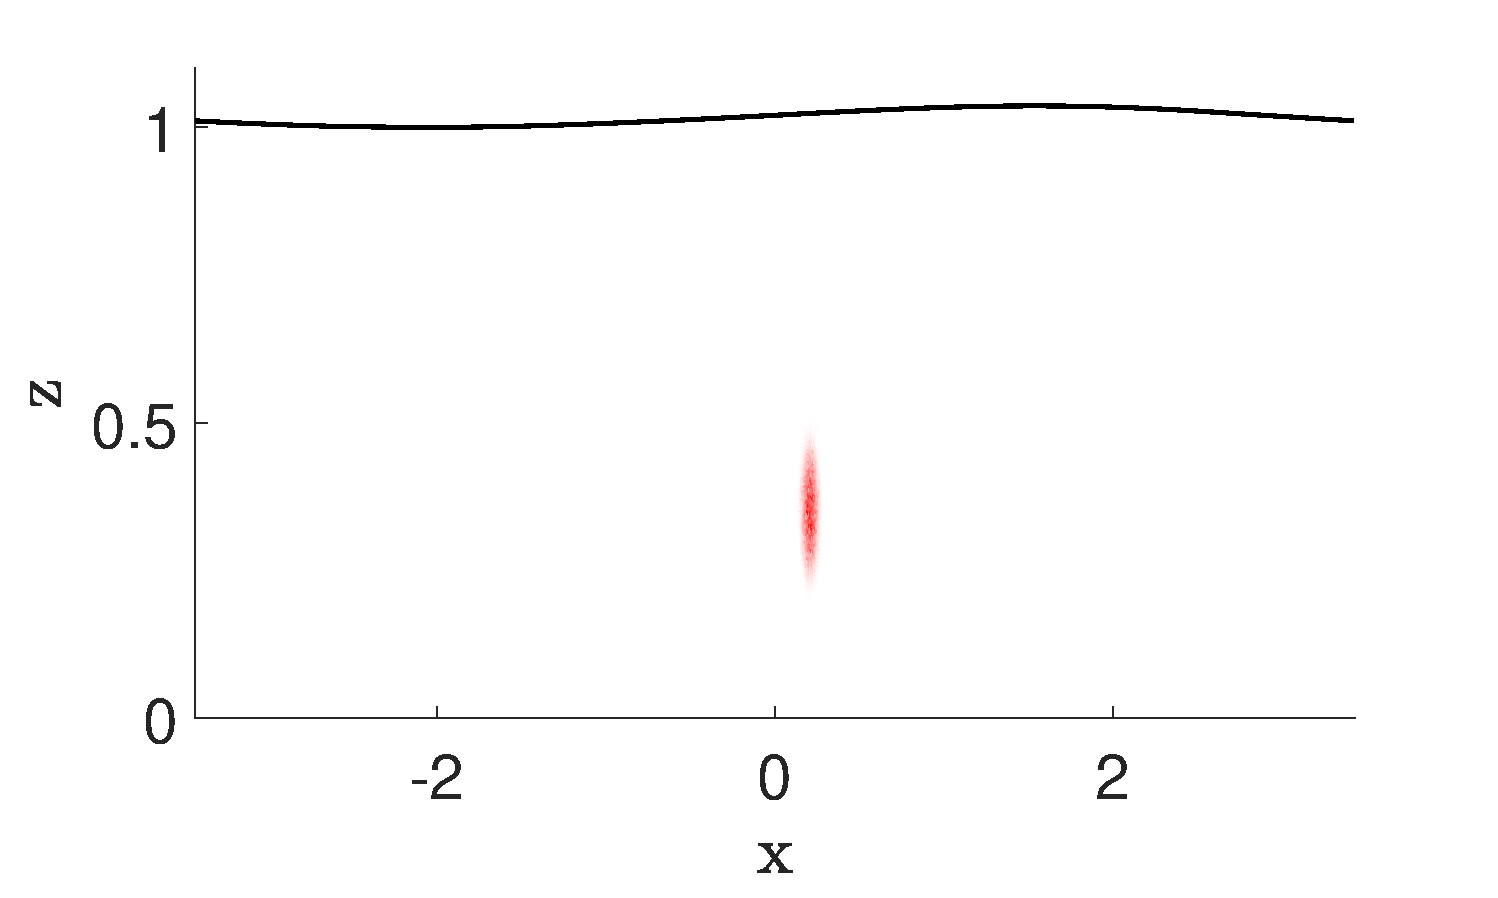
\includegraphics[width=.35\textwidth]{wave_over_vortices_m_pt3_w0_1} & 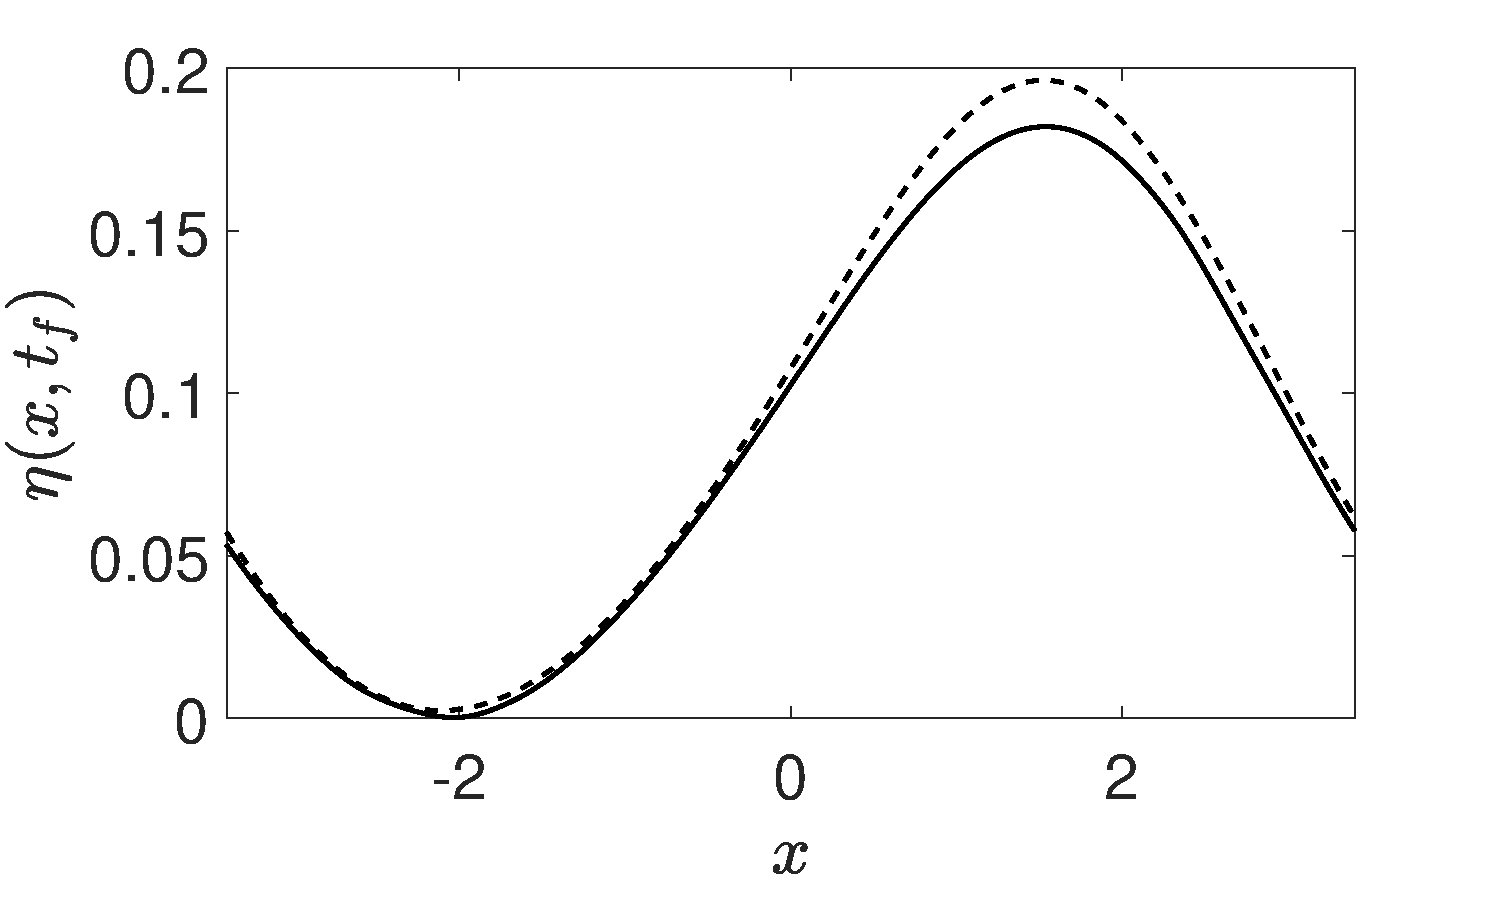
\includegraphics[width=.35\textwidth]{profiles_m_pt3_w0_1}\\
(a)  $F=.01$ & (b)  $F=.01$\\
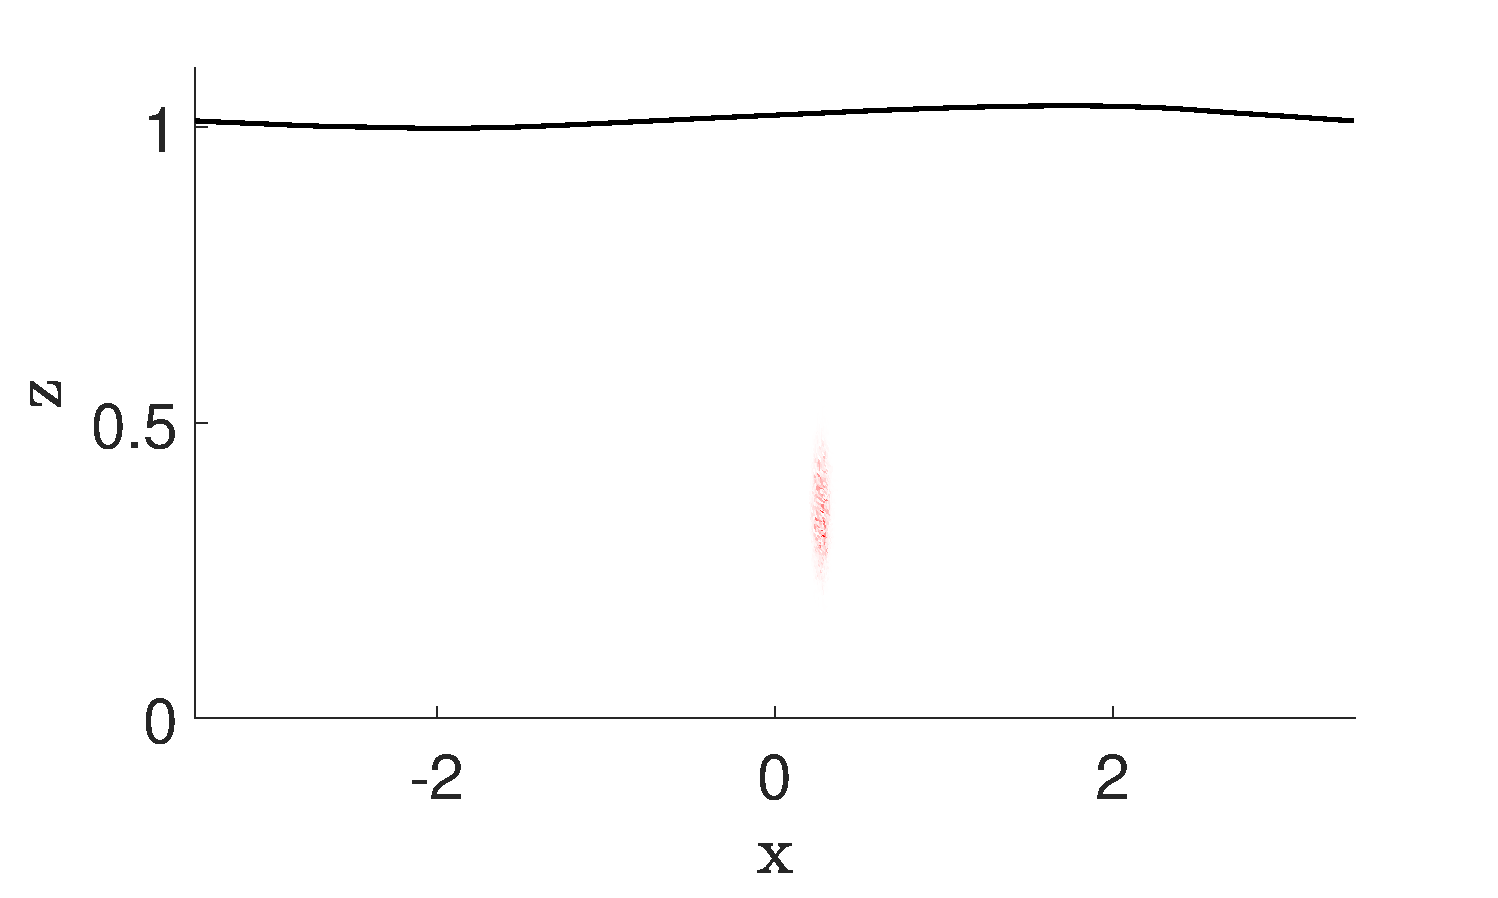
\includegraphics[width=.35\textwidth]{wave_over_vortices_m_pt3_w0_5} & 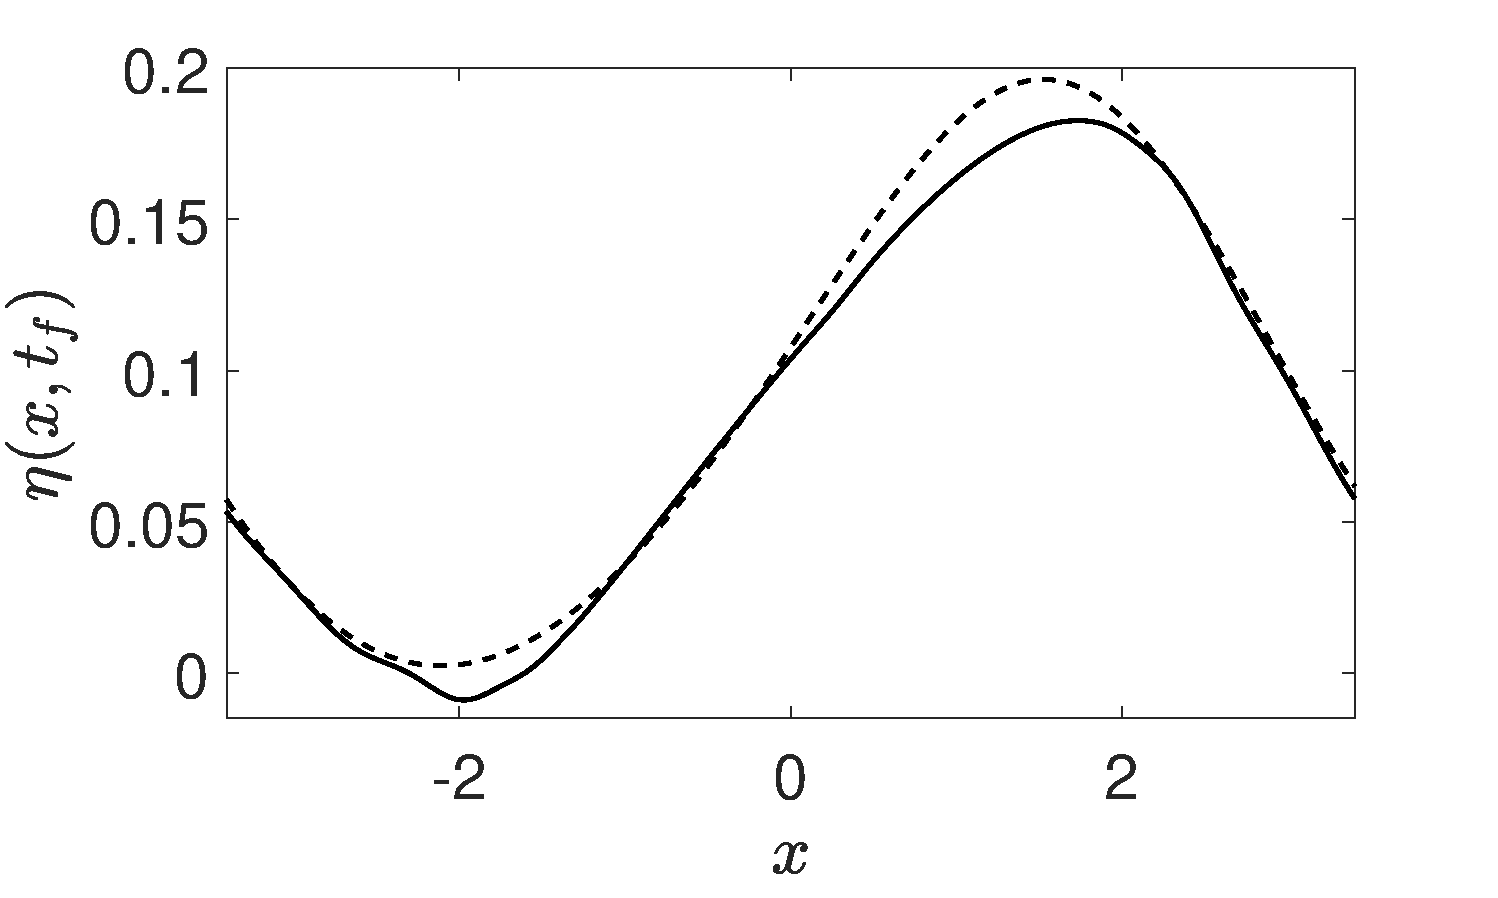
\includegraphics[width=.35\textwidth]{profiles_m_pt3_w0_5}\\
(c)  $F=.05$ & (d)  $F=.05$\\
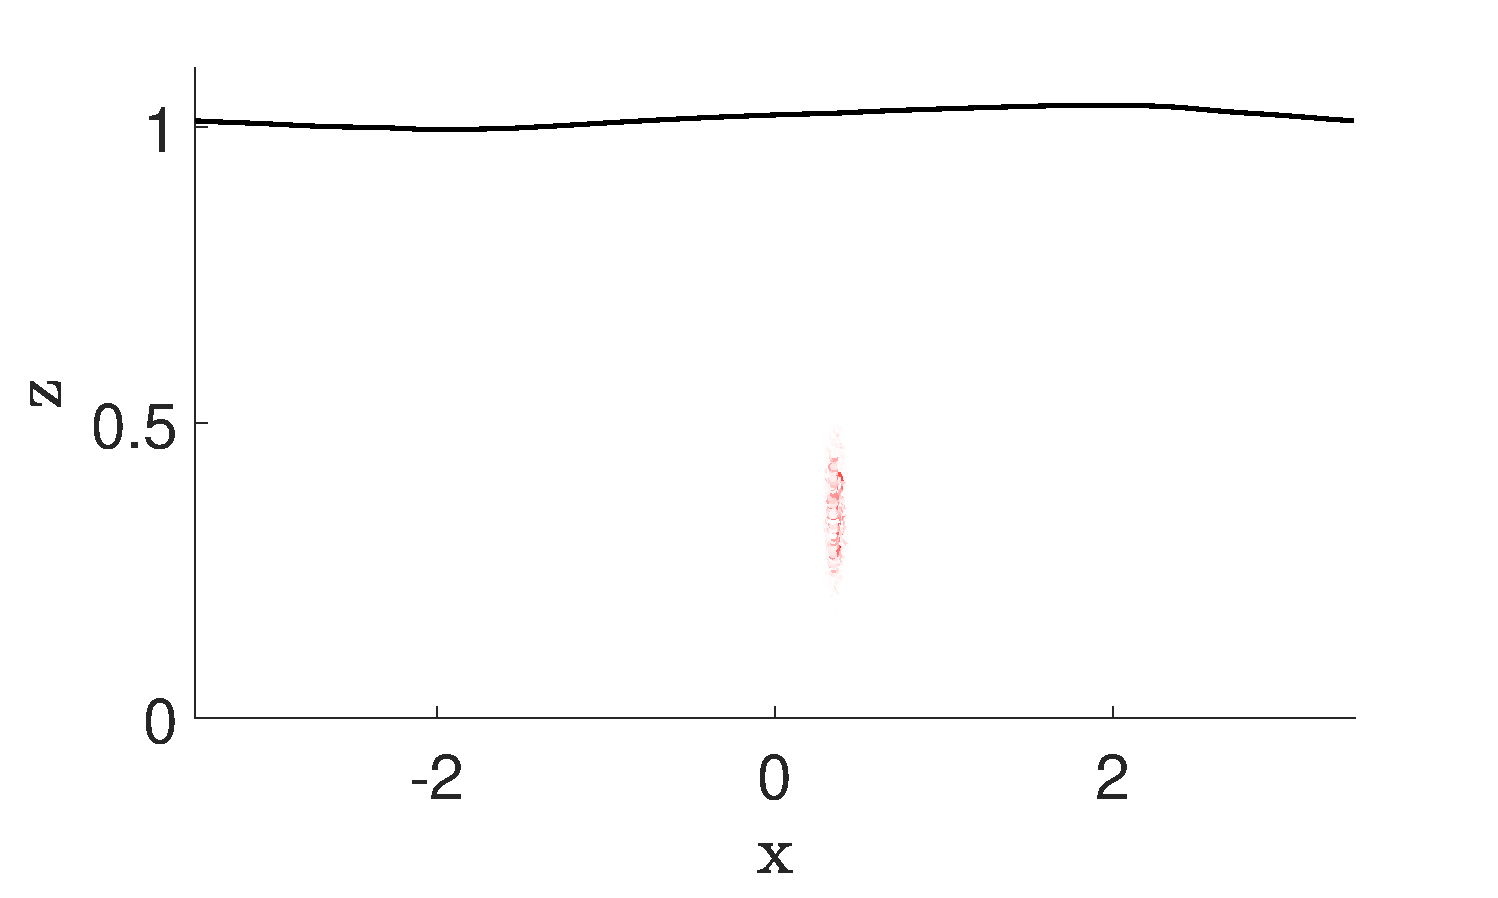
\includegraphics[width=.35\textwidth]{wave_over_vortices_m_pt3_w0_10} & 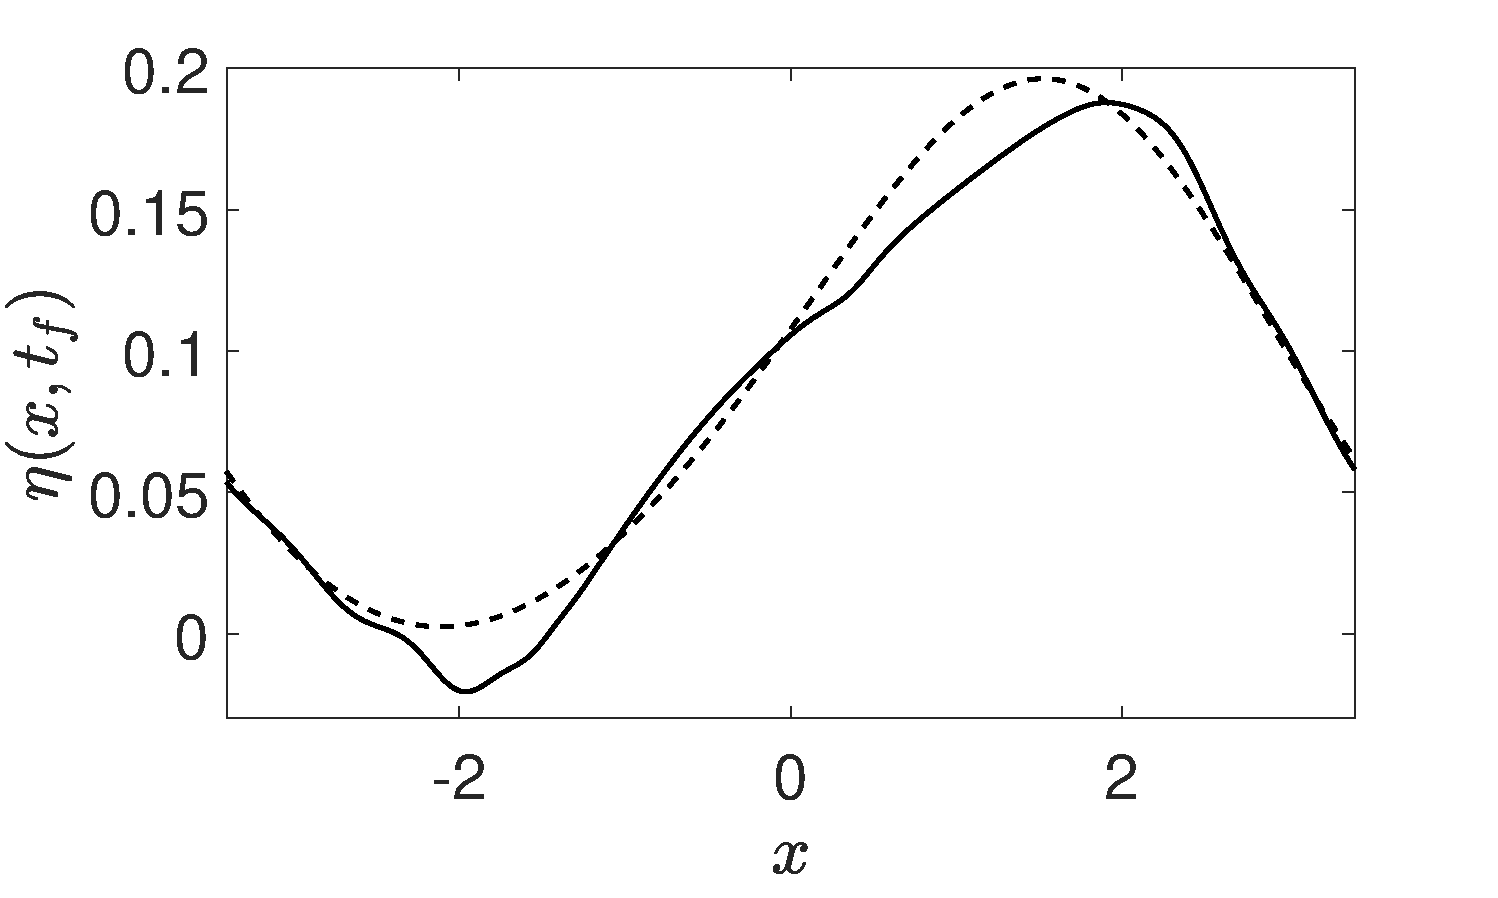
\includegraphics[width=.35\textwidth]{profiles_m_pt3_w0_10}\\
(e)  $F=.1$ & (f)  $F=.1$
\end{tabular}
\caption{Waves over the vortex patch are shown on the left for various values of Froude number $F$, while comparisons of a cnoidal wave over a vortex patch(-) to a cnoidal wave over an irrotational fluid (--) are shown on the right.  Here $\mu=.2$, $\gamma=\sqrt{\mu}$, $t_{f}=2/\mu$, $\tilde{m}=.3$, $\kappa = .5$; vortex spacing is kept at or near $.007$.}
\label{fig:lowsolwave}
\end{figure}

\subsection*{Elliptic Modulus $\tilde{m}=.6$}
Taking $\tilde{m}=.6$, we find that $\kappa = .43$, this corresponds to $M \approx 4.4$.  Taking $K_{T}=512$, this gives $\delta x = .0172$.  The unscaled amplitude of the cnoidal initial conditions is given by $8(\tilde{m}\kappa)^{2}\approx .53$.  As seen in Figure \ref{fig:midsolwave}, we see that the larger elliptic modulus and larger amplitude makes the surface wave less responsive to the impact of vorticity.  Nevertheless, the patch consistently lowers maximum amplitudes, and when large enough, induces significant oscillations in the surface profile.  
\begin{figure}
\centering
\begin{tabular}{cc}
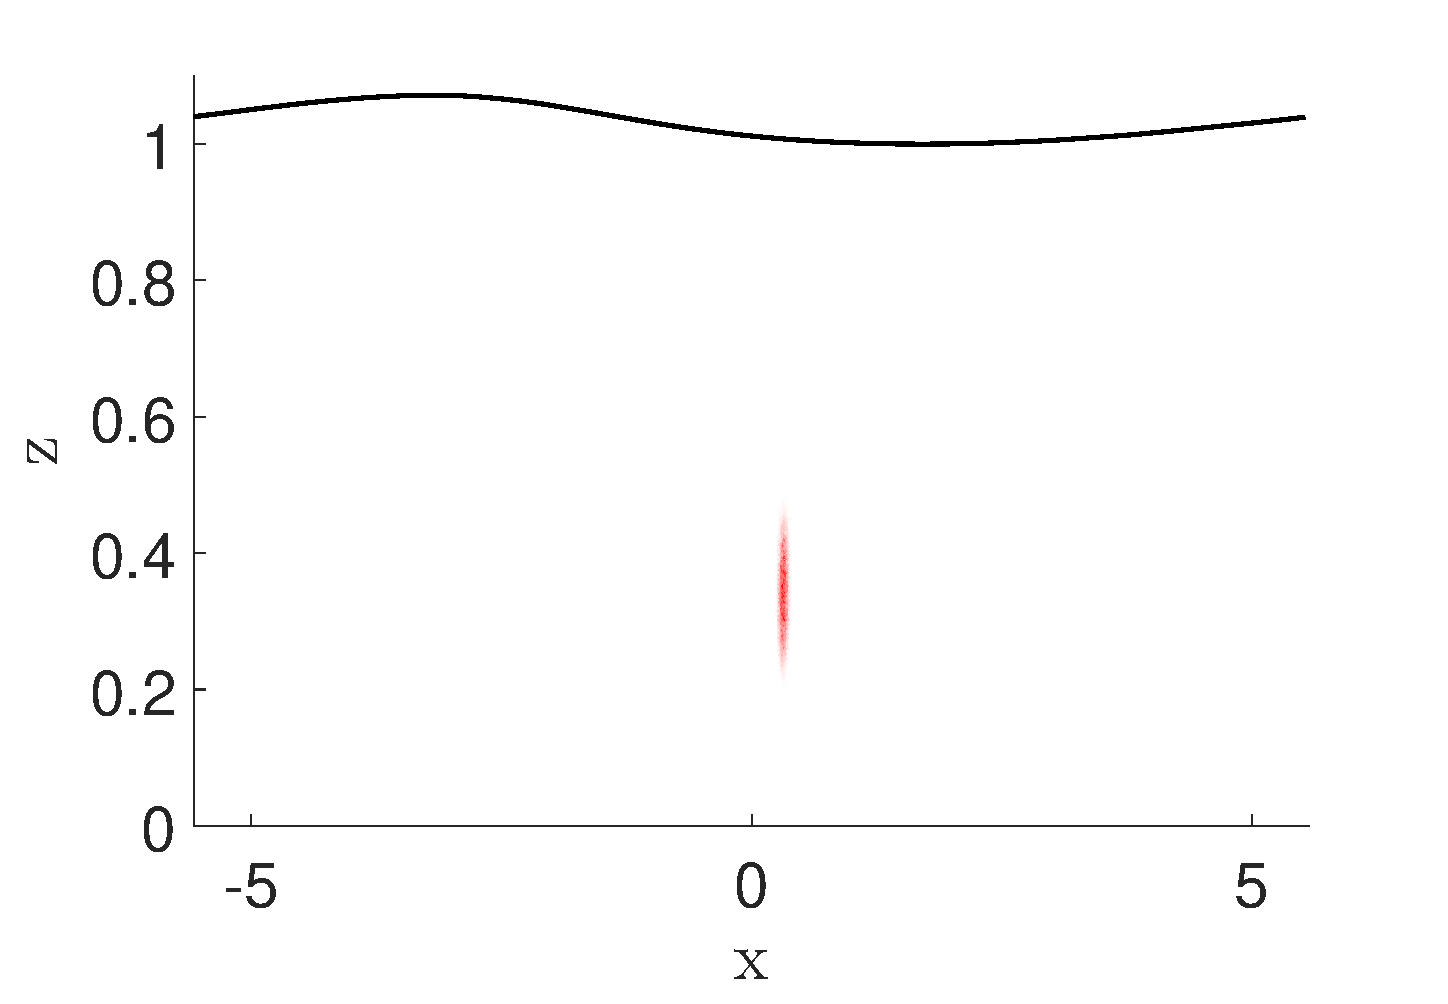
\includegraphics[width=.35\textwidth]{wave_over_vortices_m_pt6_w0_1} & 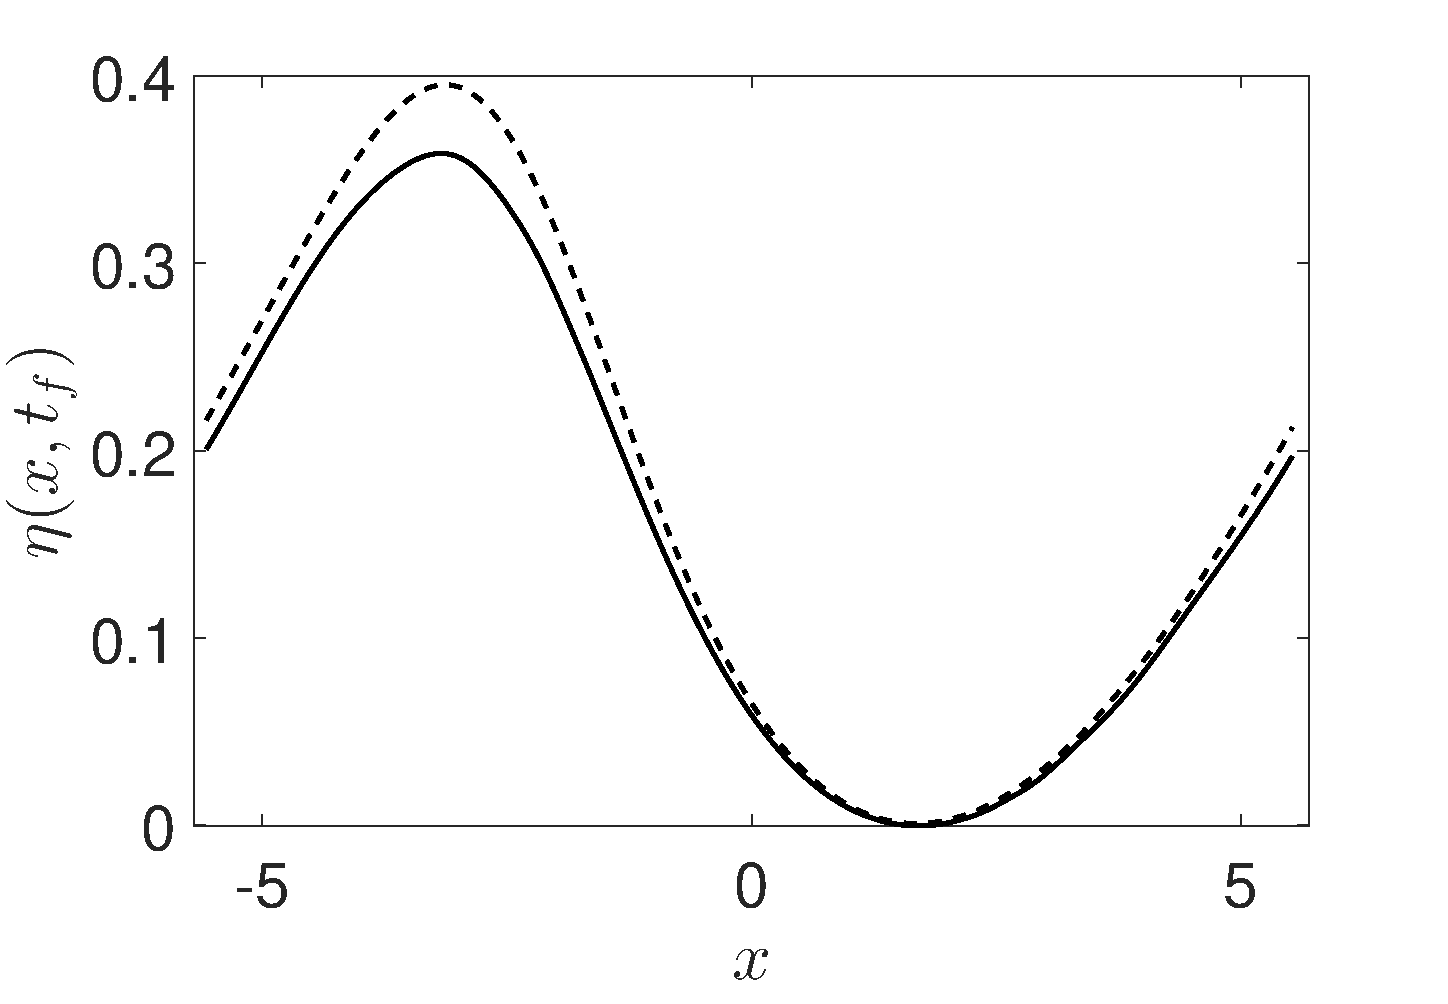
\includegraphics[width=.35\textwidth]{profiles_m_pt6_w0_1}\\
(a)  $F=.01$ & (b)  $F=.01$\\
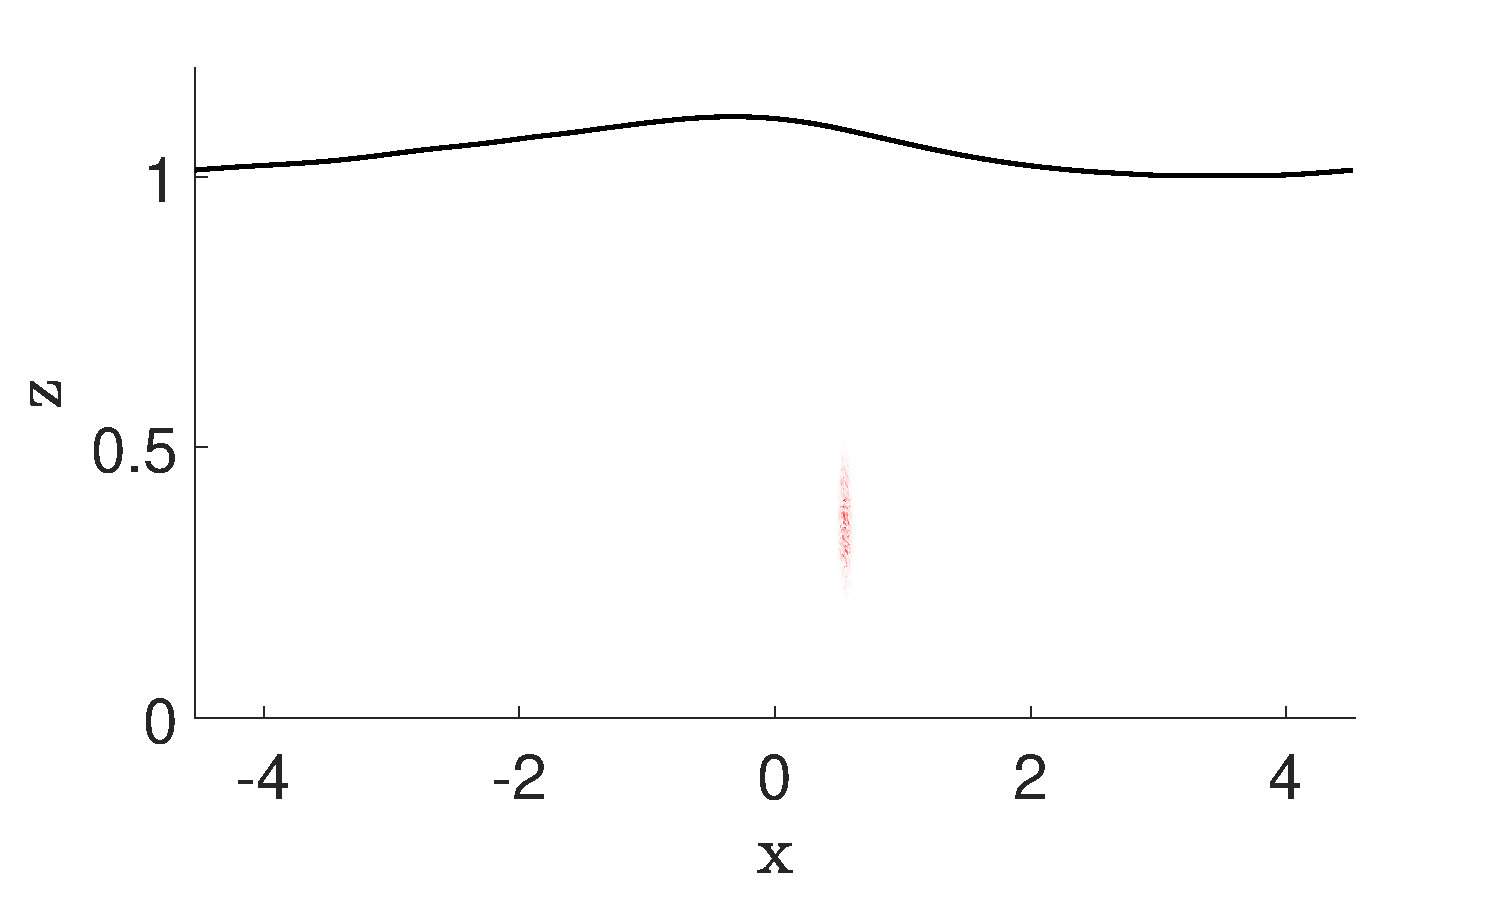
\includegraphics[width=.35\textwidth]{wave_over_vortices_m_pt6_w0_5} & 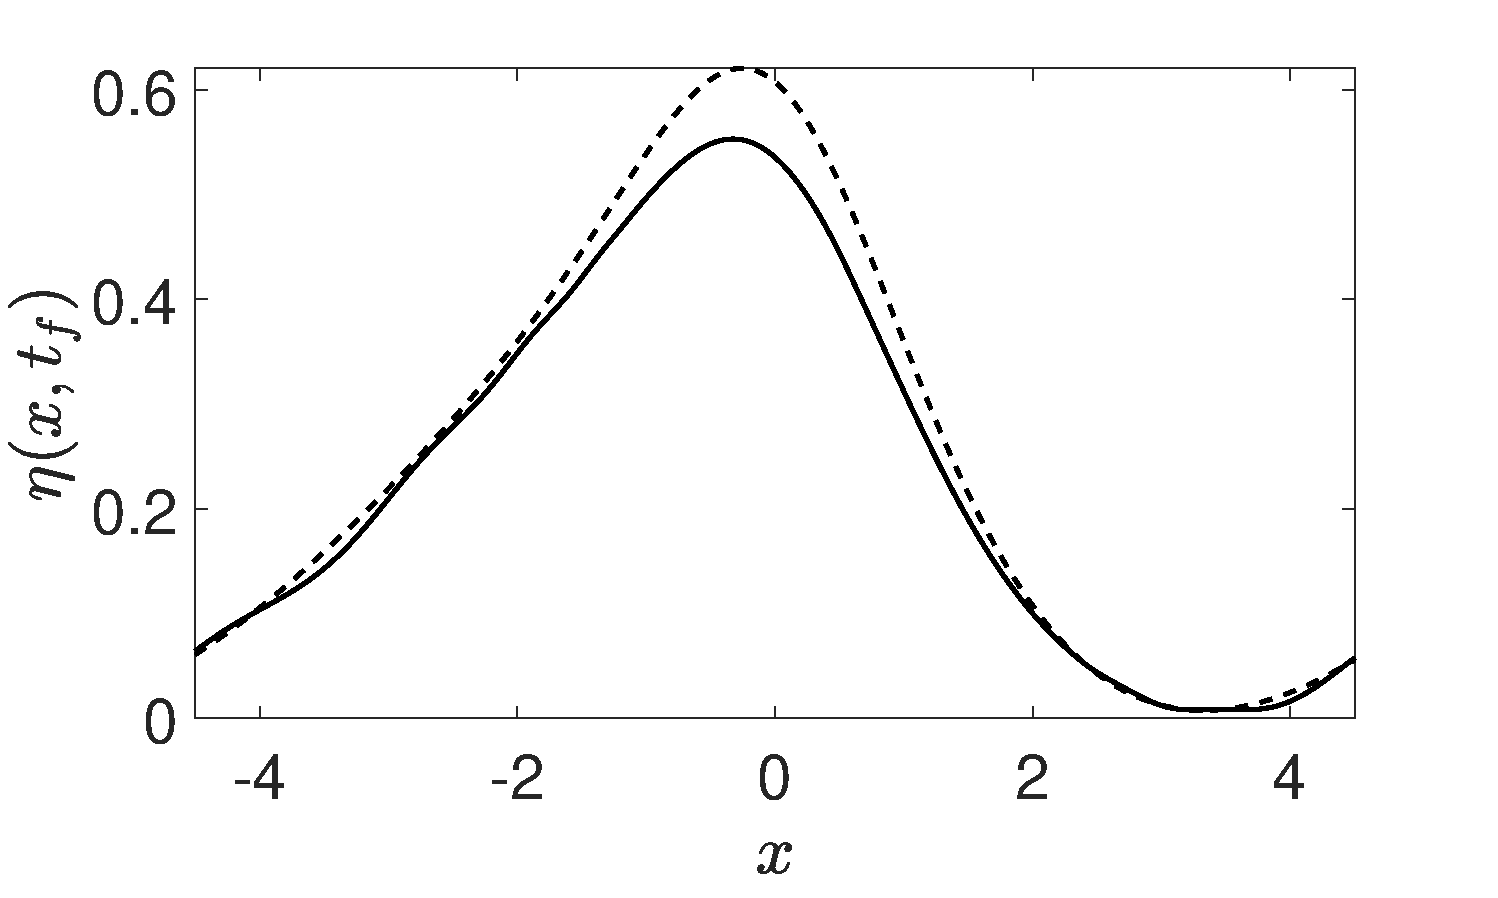
\includegraphics[width=.35\textwidth]{profiles_m_pt6_w0_5}\\
(c)  $F=.05$ & (d)  $F=.05$\\
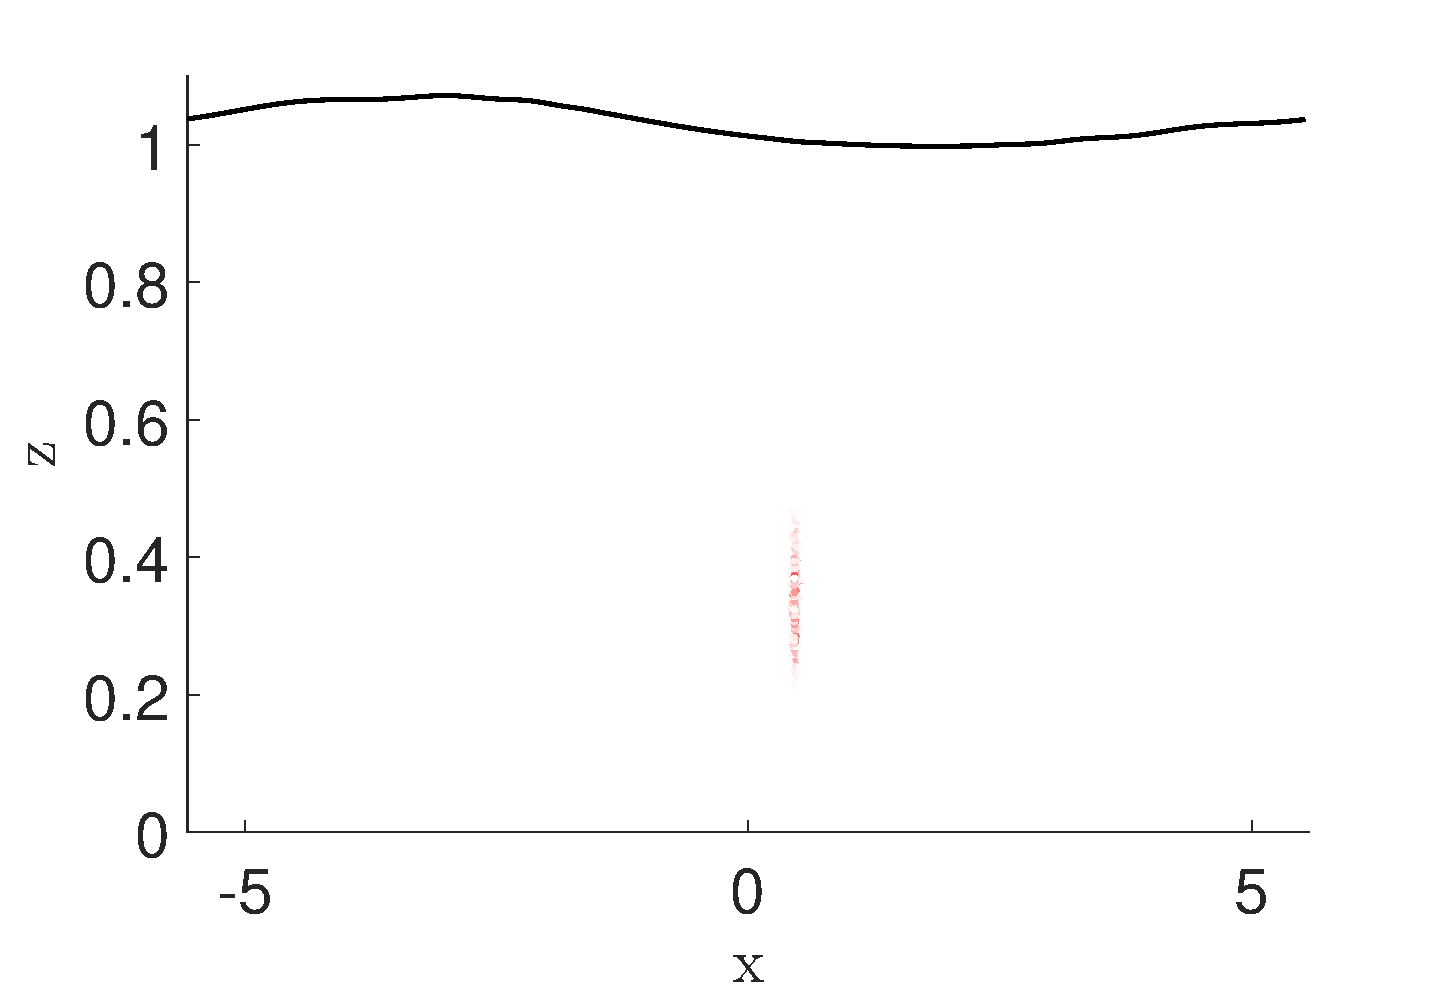
\includegraphics[width=.35\textwidth]{wave_over_vortices_m_pt6_w0_10} & 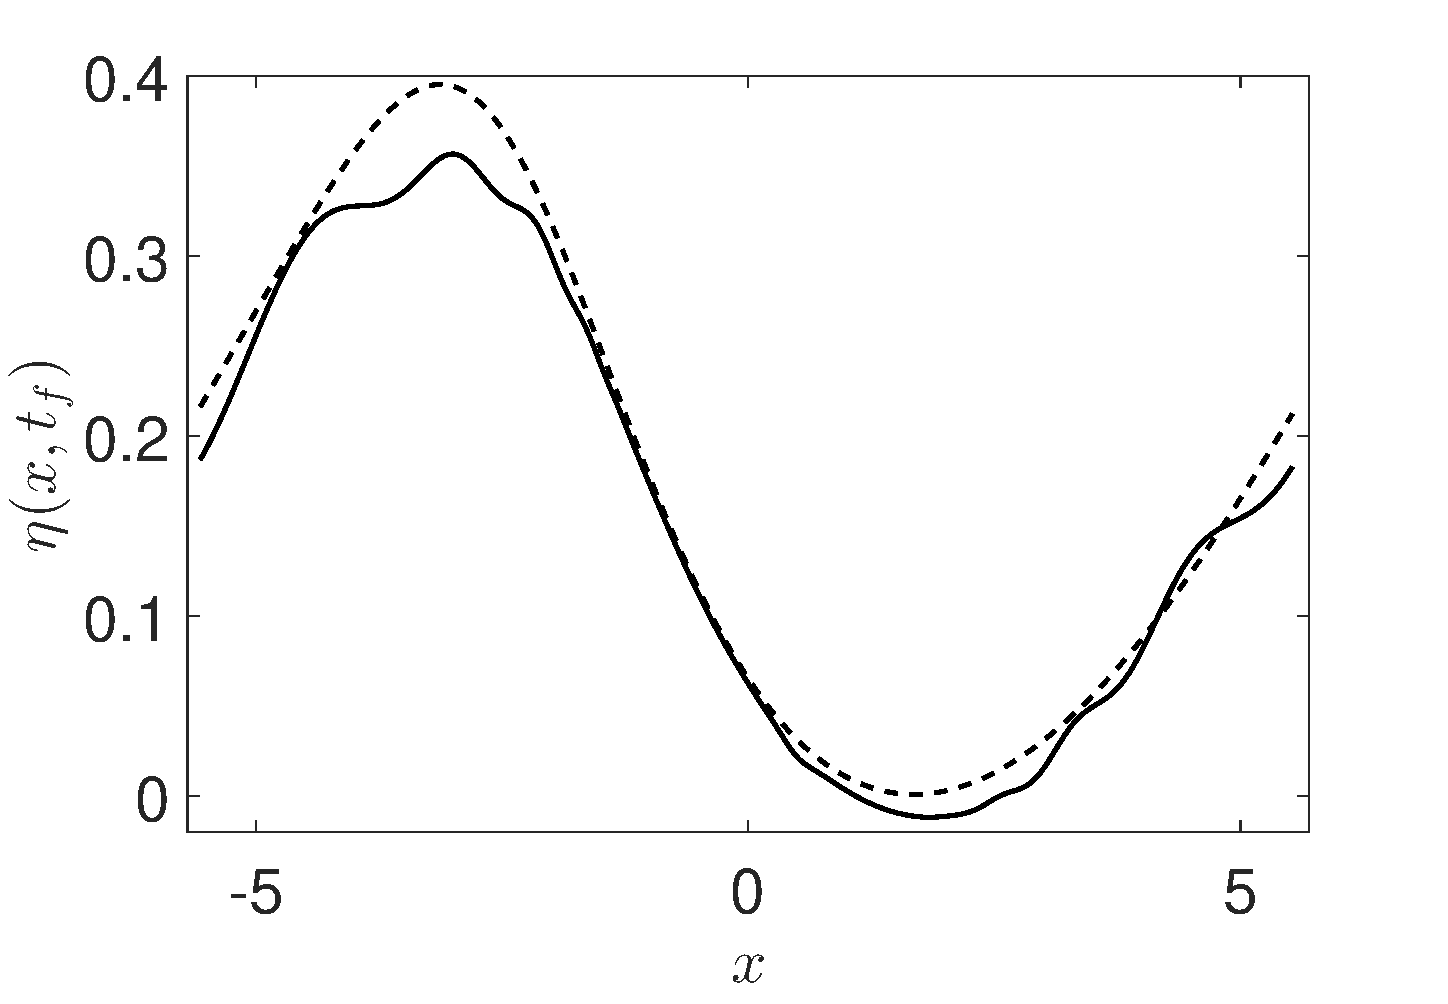
\includegraphics[width=.35\textwidth]{profiles_m_pt6_w0_10}\\
(e)  $F=.1$ & (f)  $F=.1$
\end{tabular}
\caption{Waves over the vortex patch are shown on the left for various values of Froude number $F$, while comparisons of a cnoidal wave over a vortex patch(-) to a cnoidal wave over an irrotational fluid (--) are shown on the right.  Here $\mu=.2$, $\gamma=\sqrt{\mu}$, $t_{f}=2/\mu$, $\tilde{m}=.6$, $\kappa = .43$; vortex spacing is kept at or near $.007$.}
\label{fig:midsolwave}
\end{figure}

\subsection*{Elliptic Modulus $\tilde{m}=.9$}
Taking $\tilde{m}=.9$, we find that $\kappa = .35$, this corresponds to $M \approx 7.4$.  Taking $K_{T}=512$, this gives $\delta x = .029$.  The unscaled amplitude of the cnoidal initial conditions is given by $8(\tilde{m}\kappa)^{2}\approx .8$.  Thus, somewhat suprisingly, we could use the largest amplitude wave when the initial condition was closest to that of a solitary wave profile.  Likewise, aside from causing a slight broadening and thus decrease in maximum amplitude of the near solitary wave, vorticity has the least relative impact on the wave.  Thus, if we treat the $\tilde{m}=.9$ as the `most' nonlinear of the three cases examined, since this corresponds to the case closest to that of a nonlinear solitary wave, we see vorticity has the least overall impact on the most nonlinear of waves.  

With that being said, we were not able to get reliable results for vorticity strength $\omega_{0}=10$.  In this case, a secondary vortex patch formed, which, on the face of it, is not possible in a smooth flow.  Whether this is an artificat of underresolution, instability, or some other mechanism is not clear at this time and is the subject of future research.  
\begin{figure}
\centering
\begin{tabular}{cc}
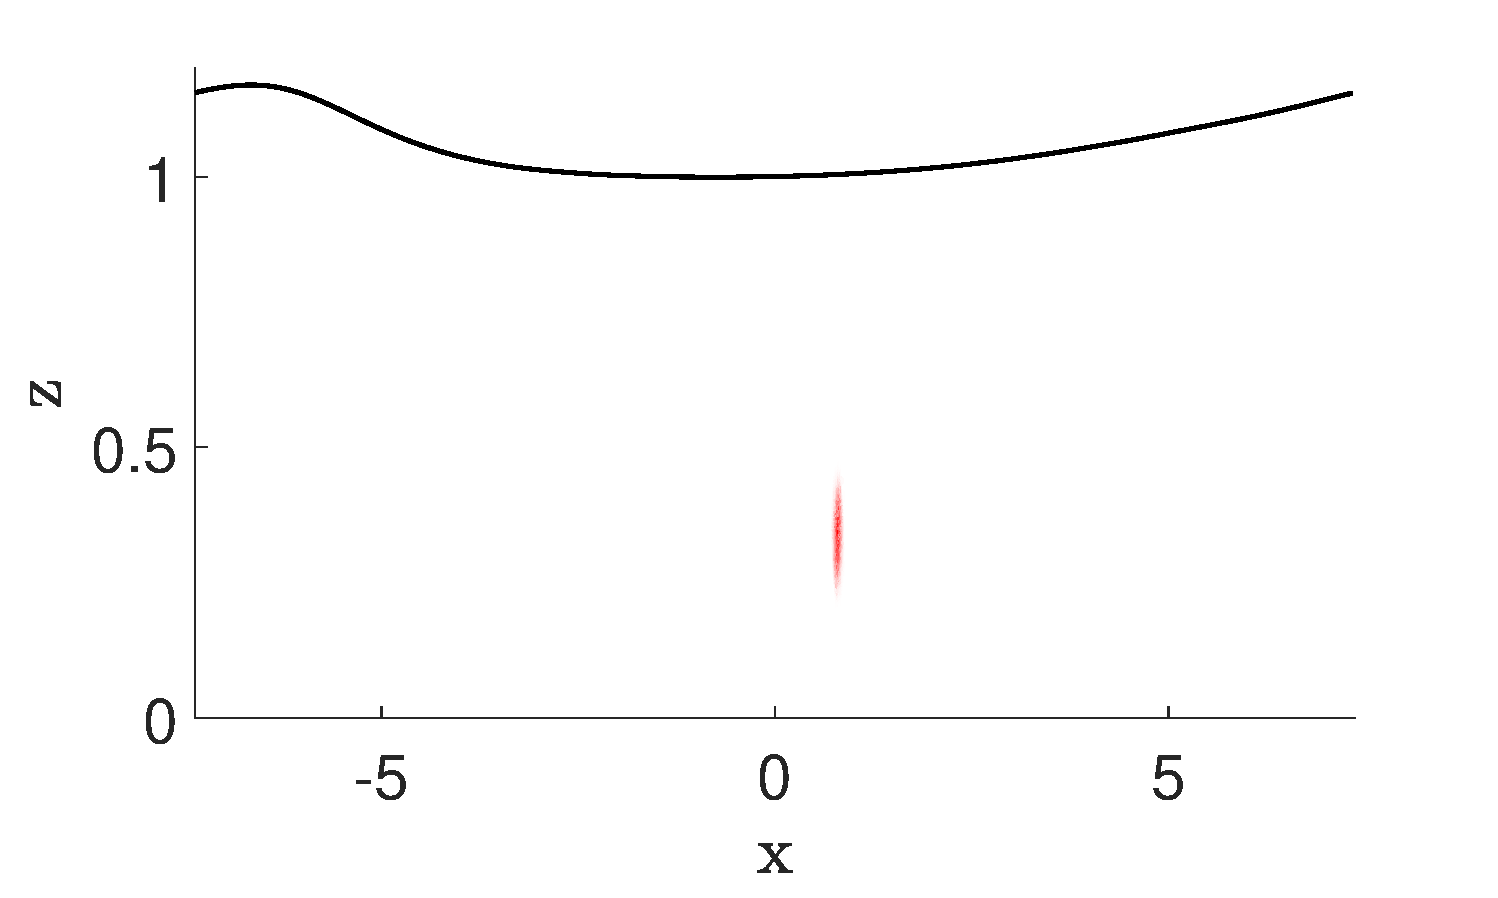
\includegraphics[width=.35\textwidth]{wave_over_vortices_m_pt9_w0_1} & 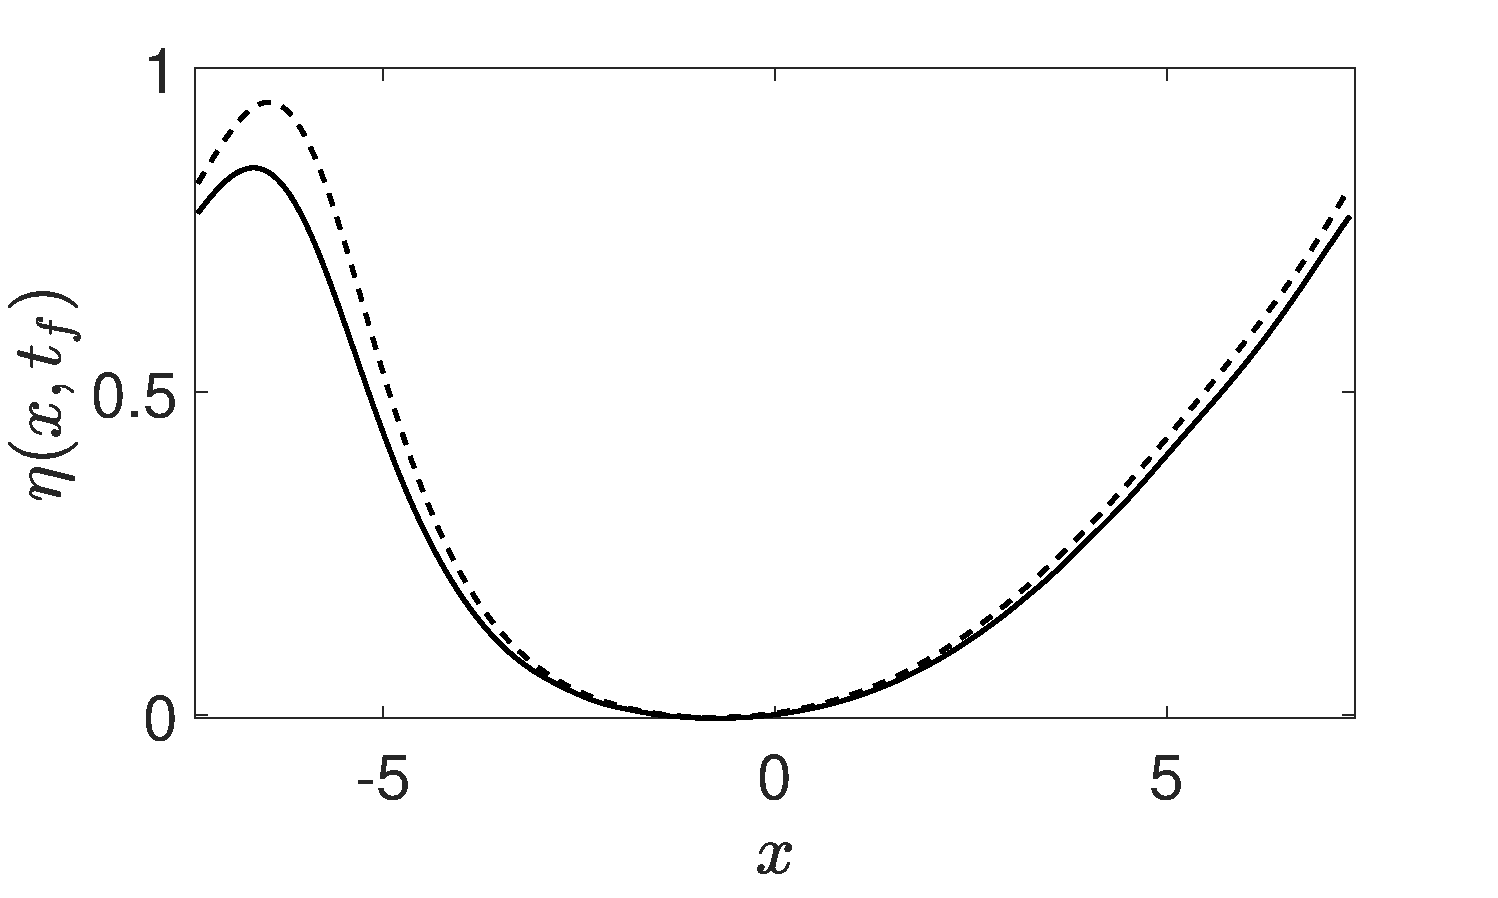
\includegraphics[width=.35\textwidth]{profiles_m_pt9_w0_1}\\
(a)  $F=.01$ & (b)  $F=.01$\\
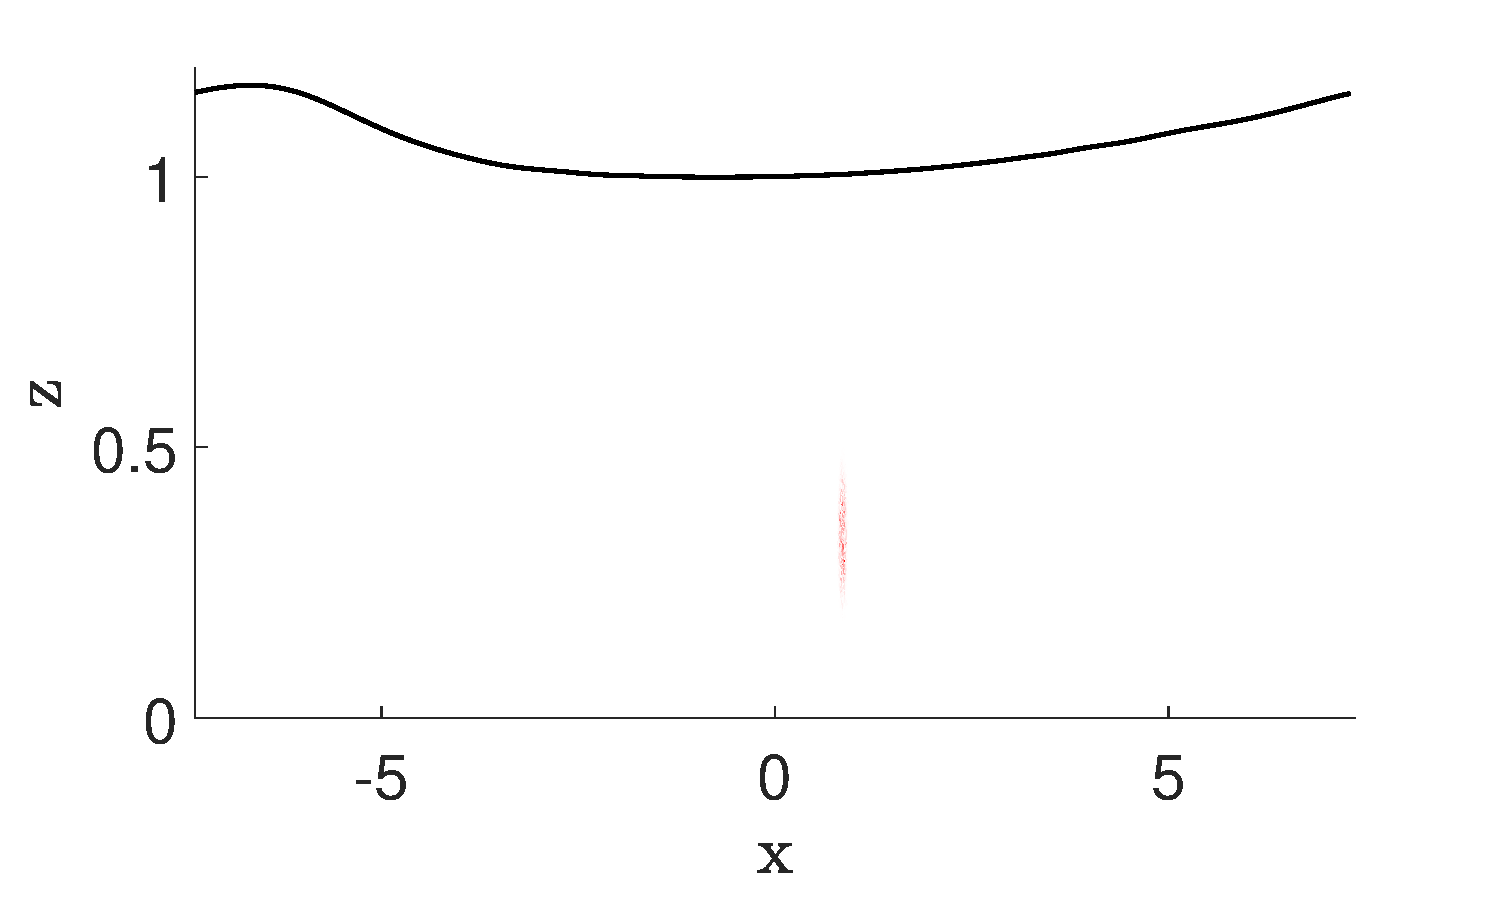
\includegraphics[width=.35\textwidth]{wave_over_vortices_m_pt9_w0_5} & 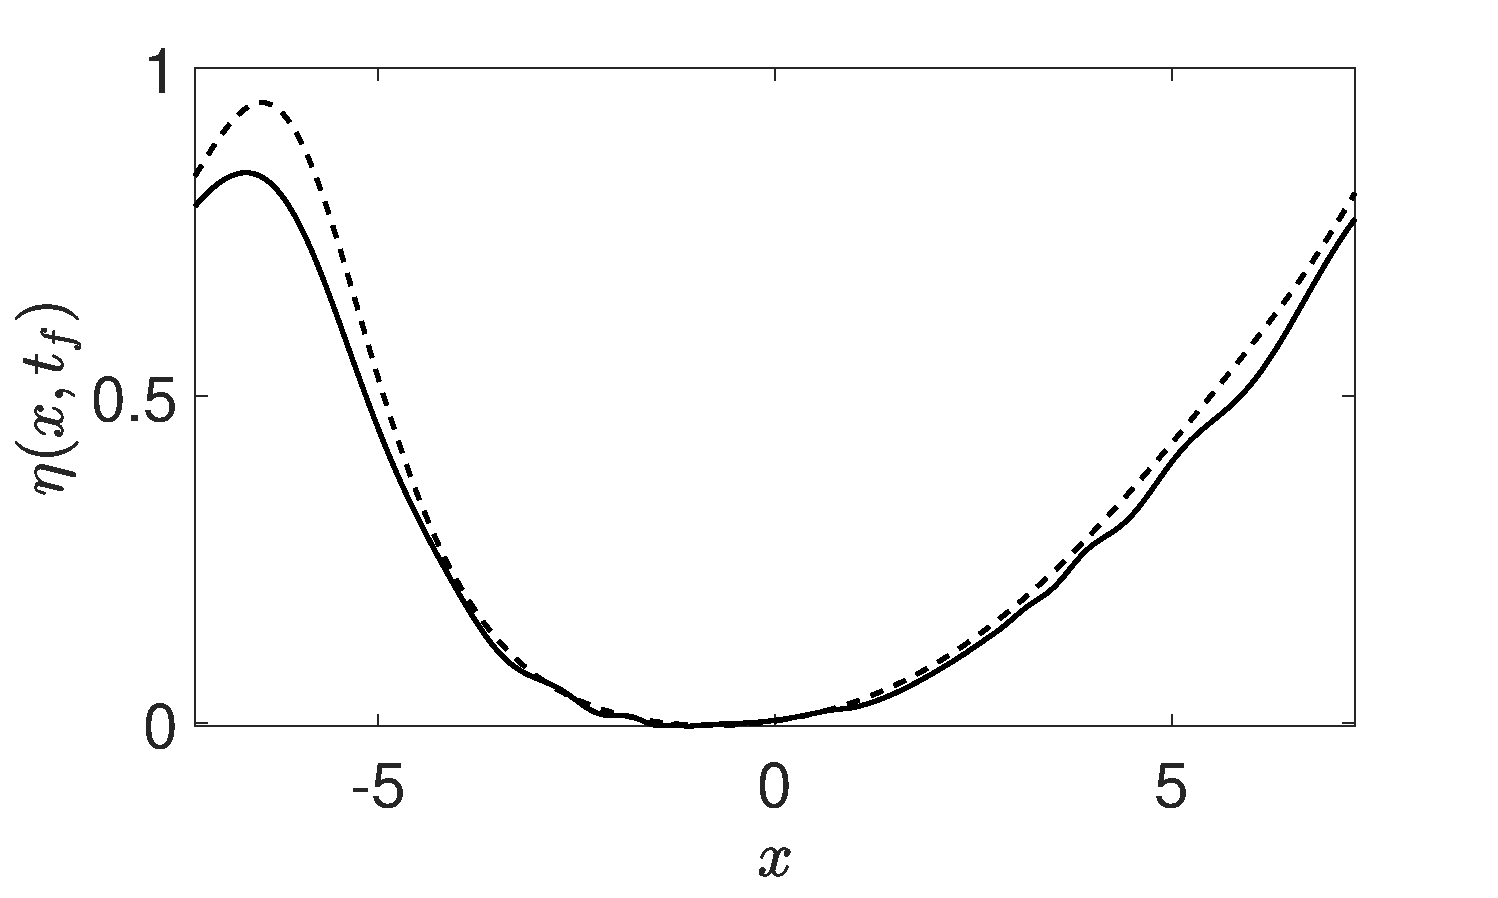
\includegraphics[width=.35\textwidth]{profiles_m_pt9_w0_5}\\
(c)  $F=.05$ & (d)  $F=.05$
\end{tabular}
\caption{Waves over the vortex patch are shown on the left for various values of Froude number $F$, while comparisons of a cnoidal wave over a vortex patch(-) to a cnoidal wave over an irrotational fluid (--) are shown on the right.  Here $\mu=.2$, $\gamma=\sqrt{\mu}$, $t_{f}=2/\mu$, $\tilde{m}=.9$, $\kappa = .35$; vortex spacing is kept at or near $.007$.}
\label{fig:highsolwave}
\end{figure}
\section*{Conclusion}
\section*{Appendix}
\bibliography{waves_over_vortices}
\bibliographystyle{unsrt}
\end{document}